%!TEX root = lomonosovReport.tex
% Добавьте ссылку на файлы с текстом работы
% Можно использовать команды:
%   \input или \include
% Пример:
%    \input{mainfiles/1-section} или \include{mainfiles/2-section}
% Команда \input позволяет включить текст файла без дополнительной обработки
% Команда \include при включении файла добавляет до него и после него команду
% перехода на новую страницу. Кроме того, она позволяет компилировать каждый файл
% в отдельности, что ускоряет сборку проекта.
% ВАЖНО: команда \include не поддерживает включение файлов, в которых уже содержится команда \include,
% т.е. не возможен рекурсивный вызов \include
\newcommand*{\Source}{
    %!TEX root = ../course_work.tex
% \phantomsection
\section{Введение} 
% \addcontentsline{toc}{section}{Введение}



Термин «первичные опухоли ЦНС» (ПО ЦНС) объединяет различные по
гистологическому строению, злокачественности и клиническому течению опухоли,
общим для которых является происхождение из тканей, составляющих центральную
нервную систему и ее оболочки. \cite{MedicTherms} \par


Опухоли головного мозга (ОГМ)- это группа различных внутричерепных новообразований 
(доброкачественных и злокачественных), возникающих вследствие запуска процесса 
аномального неконтролируемого деления клеток, которые в прошлом являлись 
нормальными составляющими различных тканей головного мозга, или возникающих 
вследствие метастазирования первичной опухоли, находящейся в другом органе. 
На возникновение новообразований влияют различные факторы: некоторые внутренние 
редкие дефекты генов, внешние воздействия - ультрафиолетовые лучи или 
рентгеновское излучение, химические вещества, инфекции, - приводят 
к спонтанному появлению мутации, что повышает риск развития 
онкологических заболеваний. Опухоли головного мозга с разными частотами затрагивают все возрастные категории 
населения. Прогноз заболевания в большинстве случаев остается неблагоприятным. Продолжительность 
жизни больных с ОГМ значительно варьируется в зависимости от типа новообразования, составляя 
в среднем от 1 года до 3-7 лет. Подобные новообразования встречаются с частотой от 5 до 7,5 
случаев на 100 тысяч начеления. Поэтому одним из наиболее значимых приоритетных направлений 
современной медицины является совершенствование существующих методов диагностики и терапии ОГМ. 
\cite{MolNeuro}


Одной из наиболее часто встречающихся 
злокачественных патологий центральной нервной
системы является глиальная опухоль. \par 

Глиомы – это собирательный термин, который объединяет все диффузные
астроцитарные и олигодендроглиальные опухоли, а также другие виды – пилоидную
астроцитому, субэпендимарную гигантоклеточную астроцитому, астробластому и
другие опухоли, исходящие из клеток глии. \cite{MedicTherms}

Опухоли ЦНС очень разнообразны. Их классифицируют по локализации, гистологическому типу, степени злокачественности.

\begin{minipage}{1.0\linewidth}
    \begin{center}
    
    \includegraphics[scale=0.07]{Astrocytoma.jpg} 
    % \caption{\scriptsize{Пайплайн для задачи предсказания выживаемости. Состоит из трех шагов:
    % сбор клинических данных, изображений и препроцессинга. Затем, выбираются извлеченные признаки и производится 
    % предсказание выживаемости.}}
\end{center}
\end{minipage}

Классификация глиом \cite{MedicTherms}:
\begin{enumerate}
    \item Астроцитома – опухоль, развивающаяся из астроцитарной части глии и
    представленная астроцитами. Может локализоваться как в больших полушариях мозга, так
    и в мозжечке, а также в стволе головного мозга и спинном мозге. Различают астроцитомы
    низкой и высокой степени злокачественности.
    \item Олигодендроглиома и олигоастроцитома – опухоли, преимущественно состоящие
    из олигодендроцитов.
    \item Глиоматоз головного мозга – это диффузное поражение глиомой структур головного
    мозга (более 3-х анатомических областей больших полушарий, обычно с переходом через
    мозолистое тело и с перивентрикулярным распространением). 
    \item Глиомы ствола головного мозга. На разных уровнях поражения ствола головного мозга
    встречаются различные глиальные опухоли. Часть этих опухолей носит доброкачественный характер и может не
    прогрессировать без лечения в течение всей жизни человека. Другие характеризуются, напротив, агрессивным течением с
    ограниченными возможностями специализированной помощи этим больным. 
   \item Глиомы спинного мозга. Как правило, диффузные интрамедуллярные опухоли,
    поражающие различные уровни спинного мозга. 
    \item и т.д.
\end{enumerate} 





Методы обследования глиальных опухолей: 
\begin{enumerate}
    \item Компьютерная томография с контрастным усилением (КТ) - это специальный метод, в котором 
    используется рентгеновское излучение. С его помощью тело человека послойно просвечивают рентгеновскими лучами. 

    \item  Магнитно-резонансная томография  с контрастным усилением(МРТ) - 
    метод визуализации, основанный на резонансе атомов водорода в организме 
    человека на магнитное поле,  создаваемое томографом.


    \item  Позитронно-эмиссионная томография  (ПЭТ) - технология визуализации, основанная на количественной и качественной оценке биохимических процессов, происходящих в тканях in vivo. 
    \item  Сцинтиграфия  - используется для оценки функционирования различных органов и тканей. Такие методы диагностики, как рентген, УЗИ, КТ или МРТ ориентированы на выявление структурных изменений в тканях организма, и не всегда способны различить болезнь на ранних её стадиях, когда отклонения проявились на уровне биохимических изменений в тканях. В это время приходит на помощь сцинтиграфия, которую поэтому и называют молекулярной диагностикой
    \item Неврологическое исследование, которое обязательно включает в себя офтальмологическую проверку остроты зрения, глазного дна и полей зрения
    \item Ангиография -  класс методов контрастного исследования кровеносных сосудов.

\end{enumerate}


На данный момент «золотым стандартом» в диагностике объемных образований головного мозга, 
определении степени злокачественности, тактики лечения и прогноза заболевания 
является магнитно-резонансная томография (МРТ) с контрастным усилением. 
Однако методы диагностики, направленные, главным образом, на оценку 
структурных изменений мозга, к которым относится и МРТ, обладают 
невысокой специфичностью в выявлении микроструктурных и  метаболических 
перестроек в опухолевой ткани, что ограничивает раннюю диагностику глиального 
образования. Накопление МР-контрастного препарата не всегда напрямую коррелирует 
со степенью злокачественности опухоли, поэтому всё чаще и чаще для диагностики применяется ПЭТ-исследование 
совместно с КТ и МРТ исследованиями для уточнения результатов. \par

Ранняя диагностика опухоли способствует высоким результатам лечения.
Заболевание нуждается в дифференцировке от гематомы внутри мозга, абсцесса,
эпилепсии, прочих опухолевых процессов в центральной нервной системе,
последствий инсульта. \par 

В настоящее время все больше внимания уделяется автоматическим методам диагностики злокачественных 
новообразований (классификация, сегментация), разработанных на основе нейронных сетей, что в перспективе 
позволит ускорить процесс диагностики патологического процесса, сокращая время между проведением исследования и началом лечения, а также уменьшить
нагрузку на врачей и медработников, которые смогут более эффективно проводить лечение заболевания.

В данной работе проводится обзор различных нейросетевых методов, которые решают задачи сегментации, классификации и 
реконструкции медицинских изображений различных моадльностей (ПЭТ, МРТ, КТ), которые могут 
применяться для автоматической диагностики злокачественных заболеваний.
Сложность работы с медицинскими данными заключается в том, что зачастую качественных наборов данных очень мало, а для разметки нужно
несколько специалистов - в некоторых случаях возникают спорные моменты
и требуется дополнительное мнение. Рассмотренные модели показали хорошие результаты производительности в своей области применения, с помощью
них можно эффективно обрабатывать, реконструировать медицинские данные, что отражает прогресс в разработке автоматических систем медицинской диагностики.




    %!TEX root = ../slides.tex
\section{Актуальность}
\begin{frame}
    \frametitle{Актуальность}
    \begin{itemize}
        \item Число глиом составляет более 60 \% от всех опухолей центральной нервной системы.
        мозга.
        \item Ранняя диагностика опухоли способствует высоким результатам лечения. Заболевание нуждается в дифференцировке от 
        гематомы внутри мозга, абсцесса, эпилепсии, прочих опухолевых процессов в центральной нервной 
        системе, последствий инсульта.
        \item Автоматическая сегментация/классификация глиальных опухолей головного мозга по ПЭТ-изображениям
        ускорит процесс дифференциальной диагностики и поможет определить вектор последующих исследований и лечения.
        
    \end{itemize}
\end{frame}
    %!TEX root = ../slides.tex
\section{Методы сегментации ПЭТ изображений}
\begin{frame}
    \frametitle{Методы сегментации ПЭТ изображений. Общая информация}
    \begin{itemize}
        \item Без ограничения общности, сегментацию изображений
        можно представлять как две связанные задачи:
        \textit{распознавание} и \textit{оконтуривание}.
        \item Внешние и внутренние факторы, значительно
         влияющие на сегментацию ПЭТ-изображений:
         \begin{itemize}
             \item проблемы, связанные с разрешением изображения
             \item многовариантность форм, текстуры и расположения патологий
             \item шум
         \end{itemize}
        
    \end{itemize}
\end{frame}

\begin{frame}
    \frametitle{Методы}
    \begin{figure}
        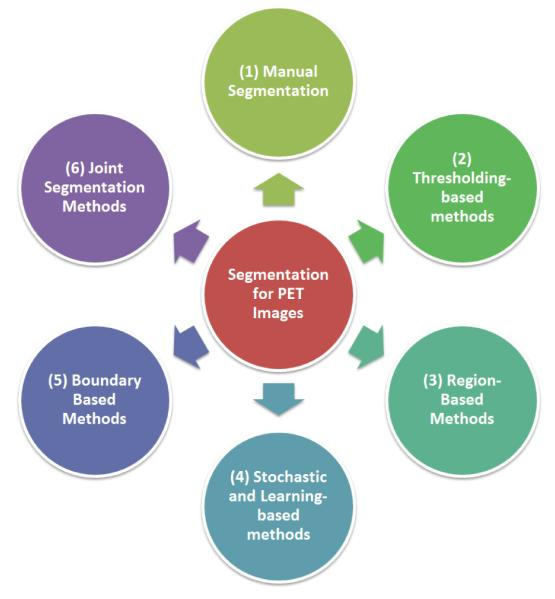
\includegraphics[scale=0.8]{cluster.jpg}
    \end{figure}
\end{frame}

%\subsection{Ручная сегментация}
%\begin{frame}
 %   \frametitle{Ручная сегментация}
  %  \begin{itemize}
   %     \item Конструирование размеченного множества изображений (ground truth)
    %    \item Оценка качества 
     %  \[DSC(V_1, V_2) = 2\frac{|V_1\cup V_2|}{|V_1|+|V_2|}\]
      % \item Сложности         
    %\end{itemize}
%\end{frame}

\subsection{Пороговые методы}
\begin{frame}
    \frametitle{Пороговые методы}
    \begin{itemize}
        \item Простой, интуитивно понятный и популярный метод,
        при котором черно-белое изображение конвертируется в бинарное, и пиксели больше определенного 
        значения считаются передним планом, а меньше - фоном.
        \item Сложность - определить оптимальное пороговое значение.        
    \end{itemize}
\end{frame}
\subsection{Стохастические модели и модели, основанные на обучении}
\begin{frame}
    \frametitle{Стохастические модели и модели, основанные на обучении}
    \begin{itemize}
        \item \textit{Mixture models} - объекты на ПЭТ-изображении
        имеют примерно гауссовское распределение и это априорное знание 
        может помочь в сегментации.
        \item \textit{Fuzzy locally adaptive Bayesian (FLAB) method} - статистический
        unsupervised метод, при котором считается, что изображение содержит два класса твердых
        тканей и конечное число \grqq нечетких уровней\glqq, которые 
        включают в себя смесь двух классов. Из-за свойства нечеткости 
        воксели принадлежат одному из двух классов, а уровень их 
        \grqq нечеткости\glqq определяется степенью принадлежности к каждому из классов.
        \item \textit{Clustering/Classification of PET image intensities}
        \begin{itemize}
            \item Классификация - разделение пространства объектов, полученного из изображения, с помощью известных меток
            \item Кластеризация - используется пространственная информацию, содержащаяся в изображениях, но без использования обучающих данных
        \end{itemize}
    \end{itemize}
\end{frame}

\subsection{Методы сегментации, основанные на регионах}
\begin{frame}
    \frametitle{Методы сегментации, основанные на регионах}
    Сегментация на основе регионов, в которых однородность 
    изображения является основным фактором для определения 
    границ объекта.
    \begin{itemize}
        \item \textit{Region Growing} - метод, который включает пространственную информацию в изображение наряду с информацией об интенсивности.
        \item \text{Графовые методы}
        \begin{itemize}
            \item Graph-cut
            \item Random walk

        \end{itemize}
        
    \end{itemize}
    
\end{frame}
\subsection{Методы выделения границ}
\begin{frame}
    \frametitle{Методы выделения границ}
    \begin{itemize}
        \item \textit{Active Contours (snakes)} - начальный контур 
        вокруг интересующего объекта деформируется и движется к желаемым границам.
        \item \textit{Level Set} - способ моделирования активных контуров путем отслеживания 
        границ между различными фазами потоков жидкости.
        \item \textit{Градиентные методы} - обычно, на границе происходит резкое изменение значения интенсивности. 
        Чтобы определить, где это происходит, вычисляется градиент между рассматриваемым вокселем и его соседями.
    \end{itemize}
\end{frame}

\subsection{Совместная сегментация}
\begin{frame}
    \frametitle{Совместная сегментация}
    \begin{itemize}
        \item Для сегментации совмещаются несколько изображений различных модальностей, 
        содержащих дополнительную информацию из входных данных. Обычно это ПЭТ/КТ и ПЭТ/МРТ.
    \end{itemize}
\end{frame}
    %!TEX root = ../slides.tex

\section{Виртуальные ПЭТ-изображения}


\begin{frame}
    \frametitle{Виртуальные ПЭТ-изображения}
    Несмотря на то, что ПЭТ-исследование имеет большое количество положительных сторон, у него имеются противопоказания и метод остается труднодоступным для некоторых категорий людей:
    \begin{itemize}
        \item радиоактивный компонент опасен для определенной категории пациентов даже в малых дозах
        \item метод дорогостоящий
        \item ПЭТ - аппараты имеются не во всех медицинских центрах, отдаленных регионах
    \end{itemize}

\end{frame}

\begin{frame}
    \begin{figure}
        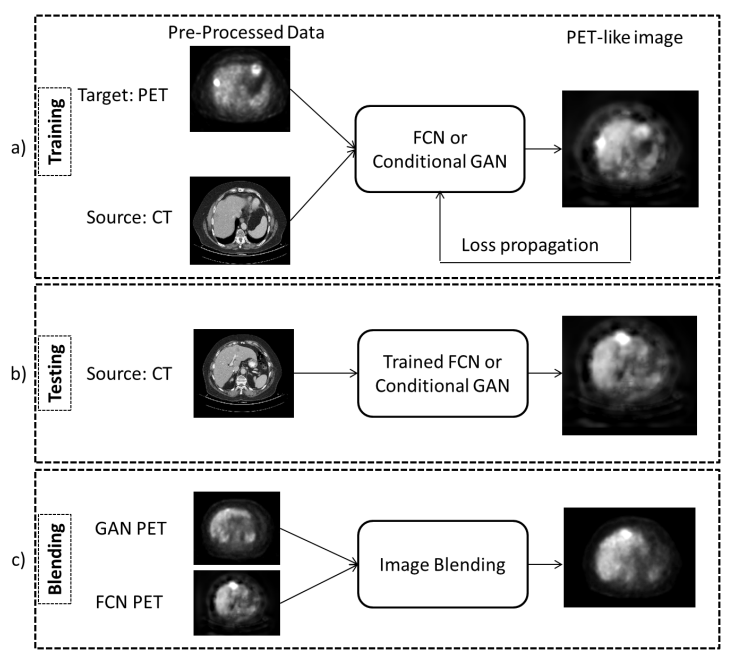
\includegraphics[scale=0.3]{virtual.png}
    \end{figure}
\end{frame}

\begin{frame}
    \begin{figure}
        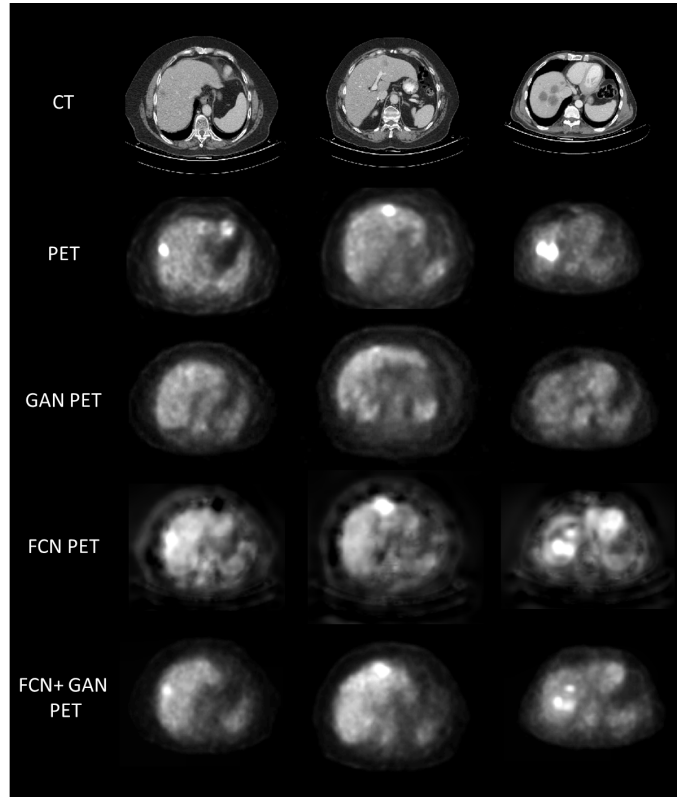
\includegraphics[scale=0.28]{virtualG.png}
    \end{figure}
\end{frame}


    \phantomsection
\section*{Заключение} 
\addcontentsline{toc}{section}{Заключение}





На сегодняшний день остро стоит проблема раннего выявления онкологических заболеваний 
головного мозга, дифференциальной диагностике от других заболеваний, последующего лечения
Методы автоматической сегментации/классификации могут ускорить процесс принятия 
решений специалистами, перечисленные методы показывают хорошую результативность, но предстоит еще 
много исследований до их внедрения в реальные медицинские системы \par


Виртуальные ПЭТ: сложно представить
их использование в реальной жизни, степень востребованности и доверия к
методу, но сама задумка интересна.




}


% Информация о годе выполнения работы
\newcommand{\Date}{%
    % 16 июня 2010 г.%
    %\today%     % Текущий день
    22 апреля 2022 г.
}

% Укажите тип работы
% Например:
%     Выпускная квалификационная работа,
%     Магистерская диссертация,
%     Курсовая работа, реферат и т.п.
\newcommand{\WorkType}{%
    % Выпускная квалификационная работа%
    % Магистерская диссертация%
    % Курсовая работа%
    % Реферат%
    %Дипломная работа%
    Доклад
}

% Название работы
%%%%%%%%%%% ВНИМАНИЕ! %%%%%%%%%%%%%%%%
% В МГУ ОНО ДОЛЖНО В ТОЧНОСТИ
% СООТВЕТСТВОВАТЬ ВЫПИСКЕ ИЗ ПРИКАЗА
% УТОЧНИТЕ НАЗВАНИЕ В УЧЕБНОЙ ЧАСТИ
\newcommand{\Title}{%
Обзор методов дифференциальной
диагностики глиальных опухолей по данным
динамических ПЭТ - исследований%
}


% Имя автора работы
\newcommand{\Author}{%
    Айрапетьянц Каринэ Арсеновна%
}

% Информация о научном руководителе
%% Фамилия Имя Отчество%
\newcommand{\SciAdvisor}{%
    Малоян Нарек Гагикович%
}
%% В формате: И.~О.~Фамилия%
\newcommand{\SciAdvisorShort}{%
    Н.~Г.~Малоян%
}
%% должность научного руководителя
\newcommand{\Position}{%
    % профессор%
    %доцент%
    % старший преподаватель%
    % преподаватель%
    % ассистент%
    % ведущий научный сотрудник%
    % старший научный сотрудник%
    % научный сотрудник%
    % младший научный сотрудник%
}
%% учёная степень научного руководителя
\newcommand{\AcademicDegree}{%
    % д.ф.-м.н.%
    % д.т.н.%
    %к.ф.-м.н.%
    % к.т.н.%
    % без степени%
}

% Информация об организации, в которой выполнена работа
%% Город
\newcommand{\Place}{%
    Москва%
}
%% Университет
\newcommand{\Univer}{%
    Московский государственный университет имени М.~В.~Ломоносова%
}
\newcommand*{\UniverAbbr}{%
    МГУ%
}
%% Факультет
\newcommand{\Faculty}{%
    Факультет вычислительной математики и кибернетики%
}
%% Кафедра    
\newcommand{\Department}{%
    Кафедра информационной безопасности%
}     

%%%% Переключите формат экрана
\newcommand{\Aspect}{%
    % 43%
    % 1610%
    169%
}
